\apendice{Documentación técnica de programación}

Poder replicar experimentos, versiones de programas, con que datos se hacen, de donde los he sacado, comentar código

\section{Introducción}
En este anexo se va a explicar todo lo necesario que tiene que saber un programador para poder replicar los experimentos de este estudio. Incluyendo versiones de los programas usados, origen de las fuentes de datos así como la estructura del código desarrollado. 

\section{Estructura de directorios}
El proyecto se estructura en una serie de directorios que contienen tanto la documentación como el material empleado en cada escenario desarrollado.
\begin{itemize}
    \item \textbf{docs}: contiene toda la información relacionada con la documentación del proyecto, como pueden ser PDFs, ficheros LaTeX o fuentes e imágenes empleadas.
    \item \textbf{Escenario 1: ingesta desde fichero en Elastic}: contiene tanto los archivos involucrados en este escenario como el \textit{dashboard} final del mismo.
    \item \textbf{Escenario 2: ingesta desde fichero con Logstash}: contiene tanto los archivos involucrados en este escenario como el \textit{dashboard} final del mismo.
    \item \textbf{Escenario 3: ingesta a través de WebSocket a Elastic}: contiene el script de ingesta de datos junto con el \textit{dashboard} final obtenido.
    \item \textbf{Escenario 4: ingesta a través de WebSocket con Logstash}: contiene el script de ingesta de datos y el archivo de configuración de Logstash junto con el \textit{dashboard} final obtenido.
    \item \textbf{Escenario 5: ingesta de data stream con MapReduce en el servidor mediante Logstash}: contiene los scripts de ingesta de datos y el archivo de configuración de Logstash junto con el \textit{dashboard} final obtenido.
    \item \textbf{Machine Learning}: contiene los scripts de ingesta de datos junto con el \textit{dashboard} final obtenido.

\end{itemize}

\section{Manual del programador}
Para el desarrollo del proyecto se han empleado una serie de programas a parte de los que conforman el ecosistema ELK. En este apartado se van a exponer las características y configuraciones empleadas en cada uno de ellos para el desarollo del proyecto.

\subsection{ElasticSearch}
Este programa se descargó desde la \href{https://www.elastic.co/es/elasticsearch}{página oficial} del software, instalando la versión 8.11.3, la cuál consiste en un archivo comprimido el cuál una vez descomprimido ya permite el uso mediante la ejecución del archivo \textit{elasticsearch.bat} alojado en el directorio \textit{bin}, el cuál si es ejecutado arrancará el servidor en el equipo, y tras unos segundos permitirá consultar su estado accediendo desde el navegador al puerto 9200, en el cuál estará corriendo el servidor de Elastic \ref{fig:elastic9200}.

\begin{figure}
    \centering
    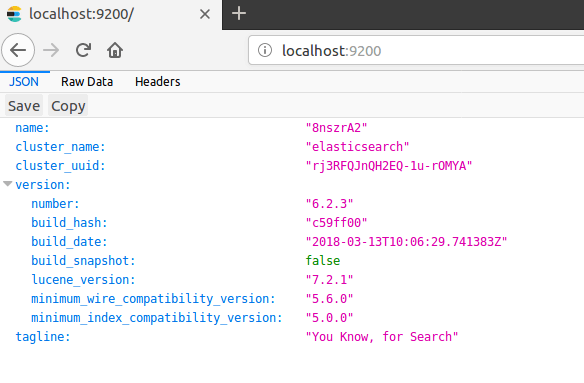
\includegraphics[width=1\linewidth]{img/elastic.png}
    \caption{ElasticSearch corriendo en el puerto local 9200}
    \label{fig:elastic9200}
\end{figure}

\subsection{Logstash}
Esta herramienta de administración de datos fue descargada desde la \href{https://www.elastic.co/es/logstash}{página oficial de Logstash}, en la versión 8.13.2, que al igual que el anterior, consistirá en un comprimido que una vez extraído se tendrá que crear un archivo de tipo .conf que será la configuración que empleará Logstash en el momento de ejecución del archivo logstash.bat ubicado en la carpeta \textit{bin}. Una vez tenemos el archivo de configuración listo ejecutaremos desde la terminal el archivo .bat mencionado anteriormente indicándole la configuración que seguirá.

\subsection{Kibana}
El útimo componente del \textit{stack ELK}, al igual que los otros dos, ha sido descargado desde la \href{https://www.elastic.co/es/kibana}{página oficial} del programa, en la versión 8.11.3, y que una vez extraído el archivo comprimido, se ejecutará el archivo \textit{kibana.bat} alojado en el directorio \textit{bin}, el cuál al ser ejecutado arrancará el programa, y tras unos segundos permitirá acceder al mismo desde el navegador en el puerto 5601, en el cuál estará corriendo el servicio de Kibana. 

\subsection{Python}
Fue instalado en su momento a través la \href{https://www.python.org/}{página oficial} con la versión 3.12.2, la cuál consiste en un ejecutable que una vez abierto instalará todos los archivo necesarios para poder escribir y ejecutar código en este lenguaje de programación.

\subsection{Jupyter Notebook}
Este programa fue descargado desde la \href{https://jupyter.org/}{página del proyecto Jupyter}, en la cuál se ofrecen diferentes programas de la empresa. en la versión 7.1.2. Una vez instalado el programa, desde la terminal se ejecuta el comando \textit{jupyter notebook} y en el puerto local 8888 se mostrará la estructura de directorios del servicio.

\subsection{Visual Studio Code}
El software que se usó para programar parte del código empleado en el proyecto fue descargado desde la \href{https://code.visualstudio.com/}{página oficial} del programa en la versión 1.90.2, y una vez ejecutado el instalador el programa estará listo para ser usado.

\section{Compilación, instalación y ejecución del proyecto}
Una vez se tiene todo el software instalado y listo, es necesario descargar los datos utilizados en el proyecto. Para ello, se deja a disposición el \href{https://github.com/hds1001/Estudio-y-configuracion-de-un-sistema-ELK}{repositorio del proyecto} en el cuál se encuentra toda la información empleada con la estructura de directorios mencionada anteriormente.

En este apartado vamos a desarrollar escenario por escenario el funcionamiento del mismo, pero lo primero antes de iniciar con el primero de ellos es tener corriendo tanto ElasticSearch como Kibana de la manera que se ha mencionado antes. Una vez la terminal muestra que ambos programas están en ejecución, se puede empezar a trabajar.

\subsection{Escenario 1: ingesta desde fichero en Elastic}
En este primer escenario, se empleó como origen de los datos un \textit{dataset} conocido en el mundo de la ciencia de datos, como es el de los pasajeros del desastre del Titanic. Este fue obtenido desde el \href{https://github.com/datasciencedojo/datasets/blob/master/titanic.csv}{repositorio} de datos \textit{Data Science Dojo}, el cuál pone a disposición pública gran variedad de \textit{datasets} para experimentar.

El \textit{dataset} consiste en un archivo de valores separados por comas con información de los 891 pasajeros del Titanic \ref{fig:titanic}, incluyendo campos como la clase del pasajero, su nombre o su edad entre otros.

\begin{figure}
    \centering
    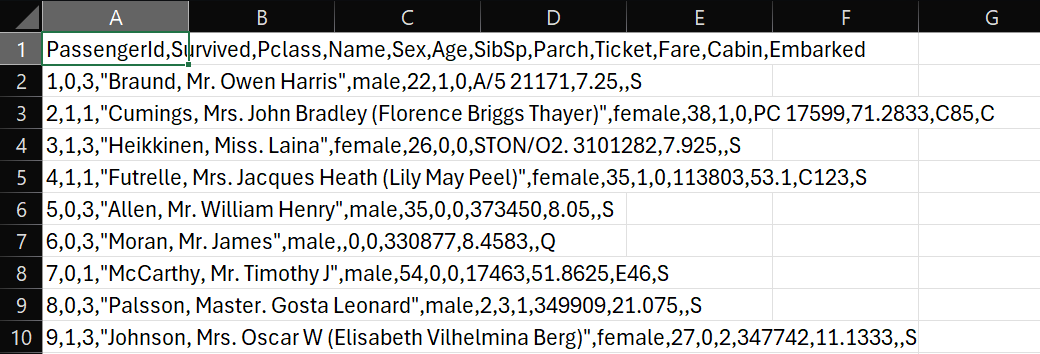
\includegraphics[width=1\linewidth]{titanic.png}
    \caption{\textit{Dataset} del titanic.}
    \label{fig:titanic}
\end{figure}

Una vez se tiene en el sistema el archivo \textit{titanic.csv}, el siguiente paso teniendo en movimiento tanto Elastic como Kibana, es importar el archivo a ElasticSearch a través de la opción \textit{Upload a file} \ref{fig:escenario11}.

\begin{figure}
    \centering
    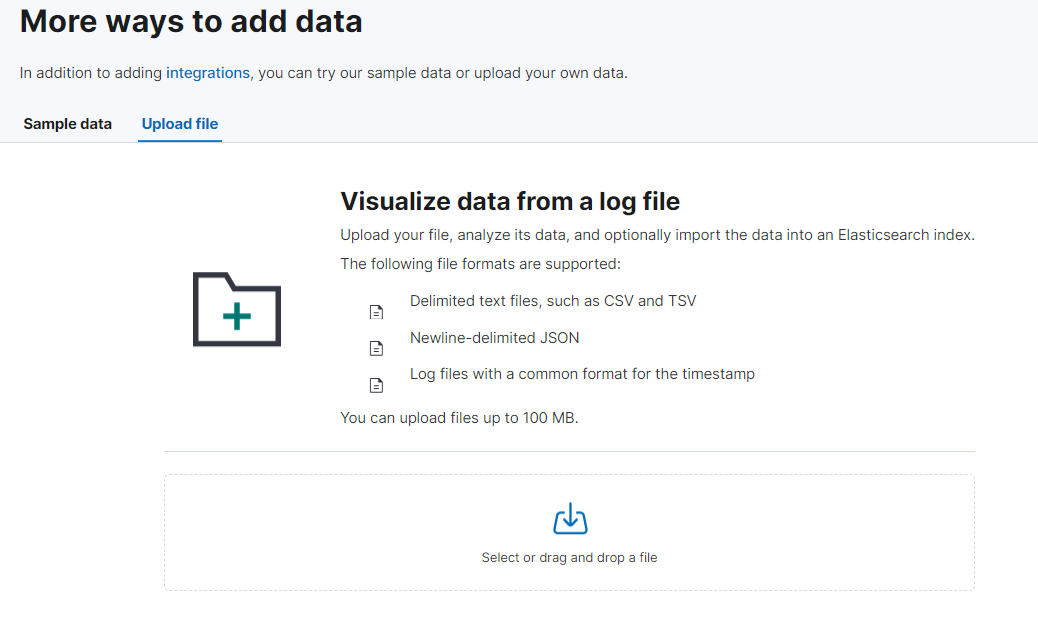
\includegraphics[width=1\linewidth]{img/ingesta1.png}
    \caption{Pantalla para importar datos del primer escenario.}
    \label{fig:escenario11}
\end{figure}

Cuando el fichero se haya cargado en ElasticSearch, se podrá comprobar desde Kibana en el apartado \textit{Discover} que todos los datos han sido cargados correctamente. Esta parte del proceso queda explicada con detenimiento en el anexo \textit{Manual de Kibana}.

\paragraph{}

\subsection{Escenario 2: ingesta desde fichero con Logstash}
Para este segundo escenario se requiere del uso de Logstash para transformar y cargar en Elastic un fichero presente en el sistema. El origen de la fuente de datos de este fichero va a ser el archivo \textit{casas.log} \ref{fig:casas}, un conjunto de datos sobre los diferentes inmuebles que se ofertan en una inmobiliaria, con información como la ciudad, el barrio o el precio entre otros.
\begin{figure}
    \centering
    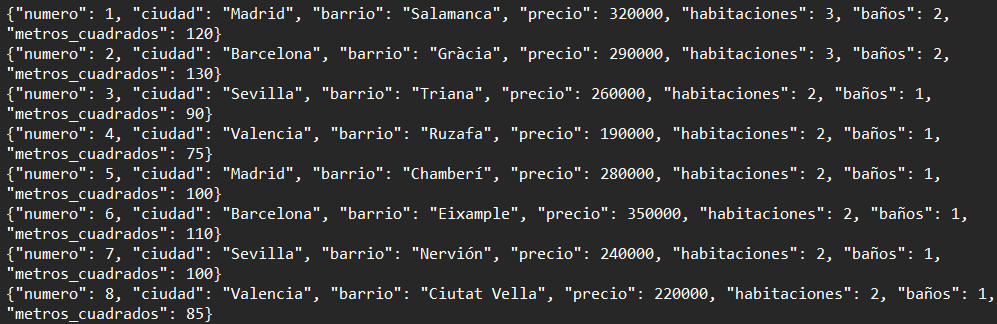
\includegraphics[width=1\linewidth]{img/casas.png}
    \caption{Estructura del fichero fuente de datos del segundo escenario.}
    \label{fig:casas}
\end{figure}

Una vez están en ejecución los otros dos componentes del \textit{stack ELK}, hay que poner en funcionamiento Logstash, pero primero se necesita un archivo que indique la configuración a seguir en este escenario, y ese va a ser el archivo \textit{escenario2.conf}, el cuál estará estructurado de manera que en el apartado \textit{input} \ref{fig:input2} se indique el \textit{path} hacia el archivo \textit{casas.log}, en la sección de filtrado \ref{fig:filter2} del archivo de configuración se realizará un mutado de los datos como se explicó en la documentación de la memoria, y en la parte de salida de los datos \ref{fig:output2} se especifica el destino, que es Elastic.

\begin{figure}
    \centering
    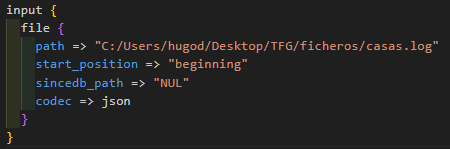
\includegraphics[width=1\linewidth]{img/input2.png}
    \caption{Apartado \textit{input} del archivo de configuración del segundo escenario.}
    \label{fig:input2}
\end{figure}

\begin{figure}
    \centering
    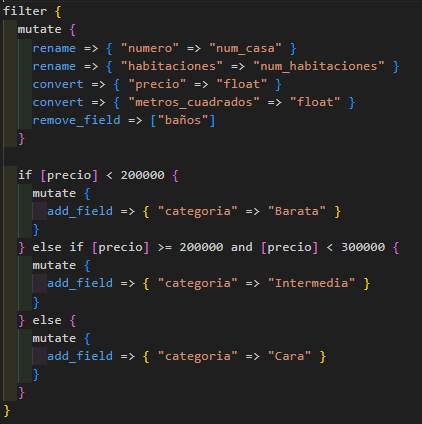
\includegraphics[width=1\linewidth]{img/filter2.png}
    \caption{Apartado \textit{filter} del archivo de configuración del segundo escenario.}
    \label{fig:filter2}
\end{figure}

\begin{figure}
    \centering
    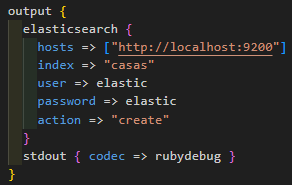
\includegraphics[width=1\linewidth]{img/output2.png}
    \caption{Apartado \textit{output} del archivo de configuración del segundo escenario.}
    \label{fig:output2}
\end{figure}

Una vez se tiene listo el archivo de configuración, desde la terminal habrá que dirigirse a la carpeta que contiene el archivo \textit{logstash-bat}, que es el directorio \textit{bin}, y desde ahi especifacar cuál es la configuración que se quiere usar en el momento de ejecución mediante el comando \textit{logstash -f escenario2.conf}. Al ejecutar se mostrarán por pantalla los datos modificados y llegarán a Elastic en dirección al índice \textit{casas}, el cuál podrá ser consultado más adelante como se indica en el \textit{Manual de Kibana}.

\paragraph{}

\subsection{Escenario 3: ingesta a través de WebSocket a Elastic}
En este tercer escenario, el origen de la ingesta de datos será un script que se suscribirá a un envío de datos en vivo por parte de la plataforma de criptodivisas \href{https://finnhub.io/docs/api/websocket-trades}{\textit{Finnhub}}. Esta suscripción se realiza a través de un WebSocket programado en Python.

Para la ejecución de este script será necesario la importación de las librerías \textit{websocket}, \textit{elasticsearch}, \textit{datetime} y \textit{json} al principio del código. Una vez importadas, en la primera parte del código\ref{fig:escenario31}, se especifica en la variable \textit{client} la dirección del puerto en el que se ejecuta el servidor de ElasticSearch. Tras esto, el método \textit{on message} define que el contenido del mensaje que se va a mandar está en formato JSON e incluirá la fecha en la que fue mandado. También indica que el contenido será mandado al índice \textit{websockets data}.
\begin{figure}
    \centering
    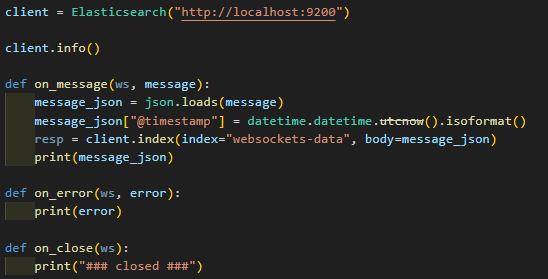
\includegraphics[width=1\linewidth]{img/escenario31.png}
    \caption{Primera parte del script de carga del tercer escenario.}
    \label{fig:escenario31}
\end{figure}

Comenzando con la segunda parte del código\ref{fig:escenario32}, en el método \textit{on open} se definen las divisas cuyo contenido va a ser incluído en el mensaje mandado a Elastic. Tras esto se define el método \textit{main} en el cuál se especificará la key de la API de \textit{Finnhub} utilizada como suscripción. También se especifica que mientrás el script esté operativo se sigan mandando datos hasta que se detenga.
\begin{figure}
    \centering
    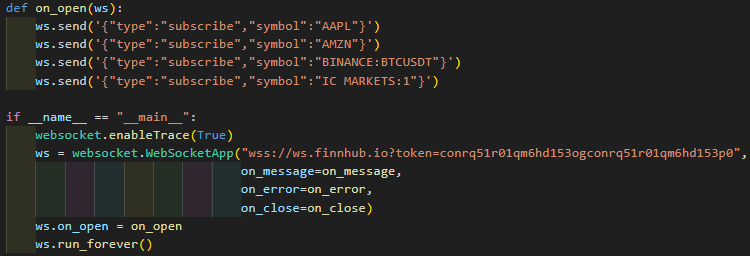
\includegraphics[width=1\linewidth]{img/escenario32.png}
    \caption{Segunda parte del script de carga del tercer escenario.}
    \label{fig:escenario32}
\end{figure}

Este script es la piedra angular de este escenario, ya que tras su ejecución los datos llegarán a Elastic y serán mostrados en el \textit{dashboard} correspondiente tal y como se mencionó en la documentación de la memoria.

\subsection{Escenario 4: ingesta a través de WebSocket con Logstash}

Para este cuarto escenario, el origen de la fuente de datos será el mismo que en el tercero, peró habrá una serie de cambios en el script de carga, de manera que en lugar de los datos ser mandados directamente un índice de ElasticSearch, serán mandado a Logstash donde se procesarán y cargarán en Elastic.

La primera parte del script de carga de datos \ref{fig:escenario41} está formada por la importación de las librerías \textit{requests}, \textit{json} y \textit{websocket}, y por el método de renombrado de campos mandados por \textit{Finnhub}, de manera que el campo que llega como \textit{s} sea mandado como \textit{Symbol}, el que llega como \textit{p} sea mandado como \textit{LastPrice}, el que llega como \textit{t} sea mandado como \textit{Timestamp}, el que llega como \textit{v} sea mandado como \textit{Volume}, y el que llega como \textit{c} sea mandado como \textit{TradeConditions} a Logstash.

\begin{figure}
    \centering
    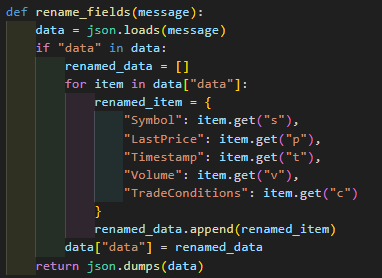
\includegraphics[width=1\linewidth]{img/websocket1.png}
    \caption{Primera parte del script de carga del cuarto escenario.}
    \label{fig:escenario41}
\end{figure}

En la segunda parte del script de carga de datos \ref{fig:escenario42}, se define el método \textit{on message} el cuál especifica que los datos serán mandados en formato JSON al puerto local 8080 en el cuál estará escuchando Logstash a la espera de información. También se definen los métodos \textit{on error} y \textit{on close} que son meramente informativos de cara la visualización del envío de datos en la terminal.
\begin{figure}
    \centering
    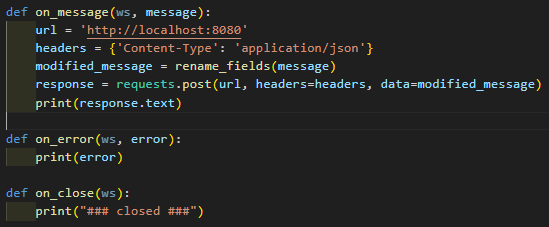
\includegraphics[width=1\linewidth]{img/websocket2.png}
    \caption{Segunda parte del script de carga del cuarto escenario.}
    \label{fig:escenario42}
\end{figure}

Para la tercera y última parte del script de carga de datos \ref{fig:escenario43}, en el método \textit{on open} se definen las divisas que se mandarán a Logstash, y en el método \textit{main} se especifica la \textit{key} empleada como suscripción al servicio de envío de datos que ofrece \textit{Finnhub}.

\begin{figure}
    \centering
    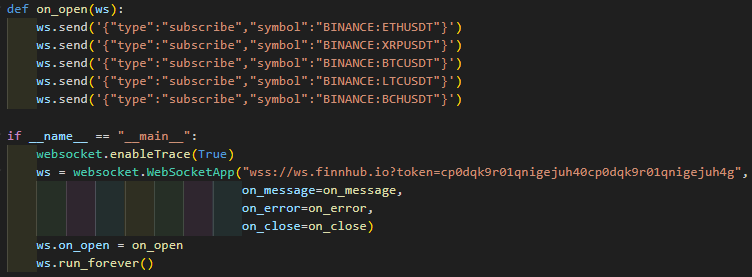
\includegraphics[width=1\linewidth]{img/websocket3.png}
    \caption{Tercera parte del script de carga del cuarto escenario.}
    \label{fig:escenario43}
\end{figure}
Una vez se ejecuta el script los datos serán mandados en forma \textit{raw} \ref{fig:salida1} al puerto local 8080, donde Logstash está a la espera de recibir datos. Una vez son mandados allí, pasan por el filtro especificado en el archivo de configuración de este cuarto escenario, el cuál esta conformado por dos partes. En la primera parte del apartado de filtrado del archivo de configuración \ref{fig:filtrado1}, se especifica que la información que va a llegar va a estar en formato JSON, que el campo \textit{TradeConditions} va a ser eliminado del mensaje final, y que el tipo del campo \textit{LastPrice} será \textit{float}, que \textit{Timestamp} será \textit{integer} y \textit{Volume} será \textit{float}.

\begin{figure}
    \centering
    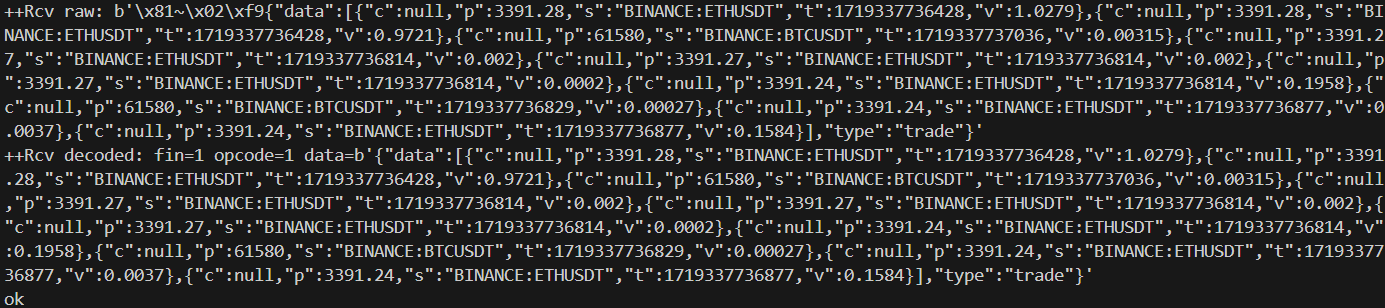
\includegraphics[width=1\linewidth]{img/salida1.png}
    \caption{Salida por pantalla de los datos del script del cuarto escenario.}
    \label{fig:salida1}
\end{figure}


\begin{figure}
    \centering
    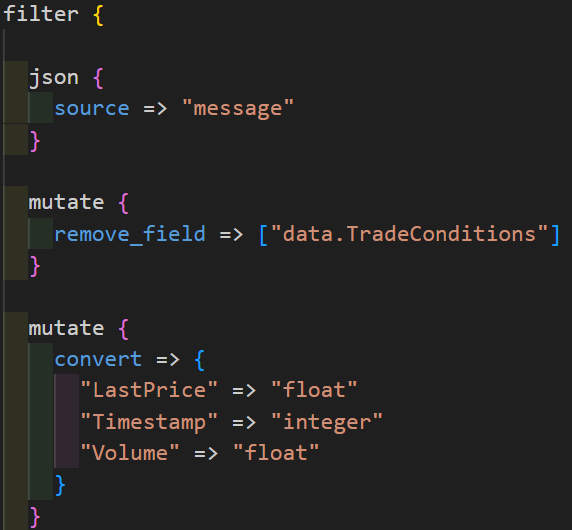
\includegraphics[width=0.5\linewidth]{escenario41.png}
    \caption{Primera parte del filtrado del archivo de configuración del cuarto escenario.}
    \label{fig:filtrado1}
\end{figure}


En la parte final del filtrado del archivo de configuración \ref{fig:filtrado2}, una vez se tienen modificados los tipos de los campos \textit{LastPrice} y \textit{Volume}, en lenguaje \textit{Ruby} se ha programado la inserción de un nuevo campo \textit{TotalPrice} calculado a partir del producto de estos dos campos.
\begin{figure}
    \centering
    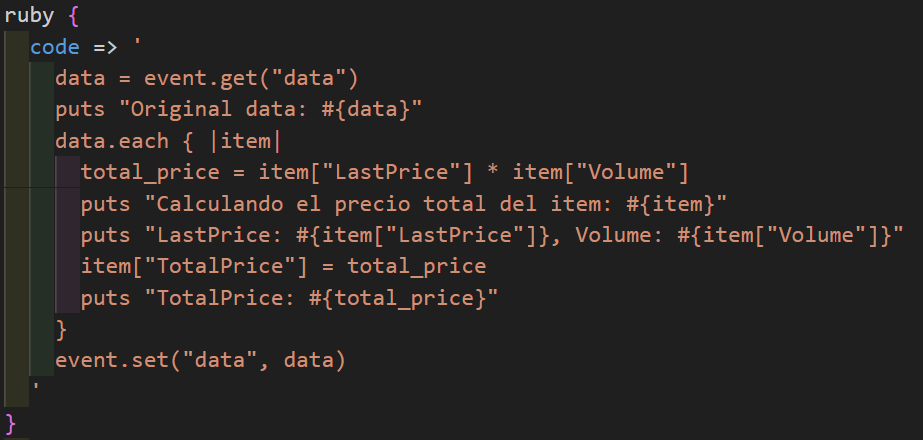
\includegraphics[width=1\linewidth]{img/escenario42.png}
    \caption{Segunda parte del filtrado del archivo de configuración del cuarto escenario.}
    \label{fig:filtrado2}
\end{figure}

Habiendo finalizado el archivo de configuración, se tienen en ejecución tanto Logstash como el script, los datos se irán mandando a Elastic con una estructura más entendible \ref{fig:salida2}.

\begin{figure}
    \centering
    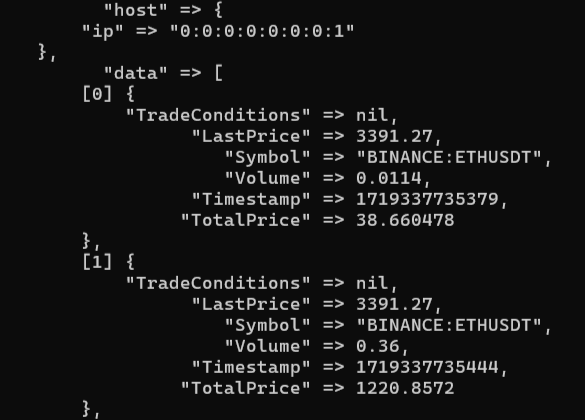
\includegraphics[width=1\linewidth]{img/salida2.png}
    \caption{Salida por pantalla de los datos una vez salen de Logstash hacia Elastic.}
    \label{fig:salida2}
\end{figure}
\paragraph{}
\paragraph{}
\paragraph{}
\paragraph{}
\paragraph{}
\paragraph{}
\paragraph{}



\subsection{Escenario 5: ingesta de data stream con MapReduce en el servidor mediante Logstash}

En este quinto escenario se pretende aplicar MapReduce a datos en vivo generados a través de un script que irá añadiendo líneas a un fichero llamado \textit{test.log} que Logstash irá leyendo y actualizando el envío de sus datos a Elastic. Este fichero contendrá información sobre las transacciones que se han hecho en un negocio, incluyendo información como el identificador del cliente, el método de pago o la categoría del producto comprado.

En la primera parte de este script generador de datos se especifica tanto la ruta del fichero destino de los datos generados, como los valores sobre los que irá operando el método generador de los datos. Para la ejecución de este script hará falta la importación de las librerías \textit{json}, \textit{random}, \textit{time} y \textit{datetime}.
\begin{figure}
    \centering
    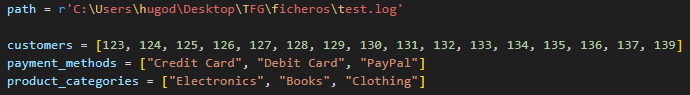
\includegraphics[width=1\linewidth]{img/escenario51.png}
    \caption{Primera parte del generador de datos del quinto escenario.}
    \label{fig:generador1}
\end{figure}

El método \textit{generate transaction} es el encargado de generar elecciones aleatorias sobre las que se han especificado previamente para los campos \textit{customer id}, \textit{amount}, \textit{payment method} y \textit{product category}. También indicará que cada línea escrita en el archivo contendrá estos campos junto a un identificador de la transacción y la fecha en la que fue generado.
\begin{figure}
    \centering
    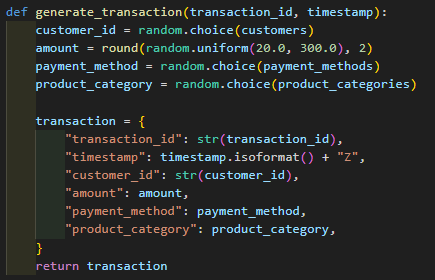
\includegraphics[width=1\linewidth]{img/escenario52.png}
    \caption{Segunda parte del generador de datos del quinto escenario.}
    \label{fig:generador2}
\end{figure}

En esta última parte del script se establece un bucle en el que comenzando por la transacción número 1 se irán generando transacciones cada segundo, y no se detendrá hasta que se pare el script.
\begin{figure}
    \centering
    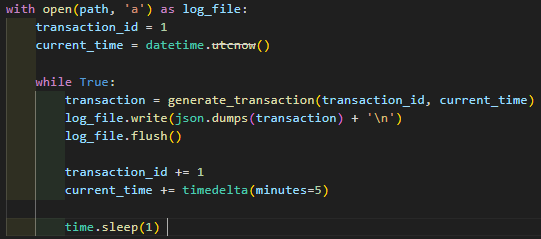
\includegraphics[width=1\linewidth]{img/escenario53.png}
    \caption{Tercera parte del generador de datos del quinto escenario.}
    \label{fig:generador3}
\end{figure}

Con esto, una vez se ejecuta el script, resultará en que el archivo \textit{test.log} irá almacenando las transacciones en un formato entendible tanto para el usuario como para Logstash.

\begin{figure}
    \centering
    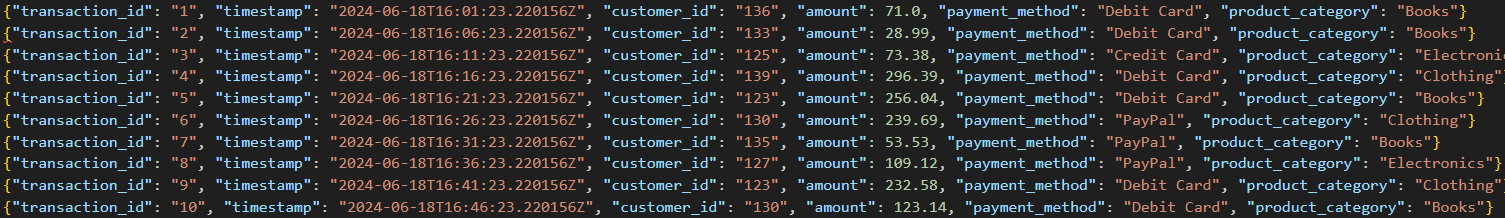
\includegraphics[width=1\linewidth]{img/salida3.png}
    \caption{Estructura de la fuente de los datos del quinto escenario.}
    \label{fig:salida3}
\end{figure}

Cuando el archivo se va llenando de líneas, se tiene Logstash en ejecución simultáneamente, de manera que se vaya ejecutando el método \textit{aggregate} tal y como se explicó en la documentación de la memoria.

\paragraph{}
\paragraph{}
\paragraph{}
\paragraph{}
\paragraph{}
\paragraph{}
\paragraph{}
\paragraph{}
\paragraph{}
\paragraph{}
\paragraph{}
\paragraph{}
\paragraph{}
\paragraph{}


\subsection{Machine Learning}

En este último caso planteado en el cuál se aplica una serie de algoritmos que ofrece la librería SKLearn sobre el popular \textit{dataset} Iris, la manera de ingestar los datos se planteó de manera que los datos de Iris estuvieran presentes en un índice en Elastic, estos datos se cargarán en el script que aplica los algoritmos, y una vez cargados cada algoritmo devolverá los datos procesados a un índice individual para cada uno.

Para resolver esta estructura planteada, se generaron dos scripts. En el primero de ellos se crea un índice en Elastic que contiene el \textit{dataset} Iris. Son necesarias las librerías \textit{pandas}, \textit{sklearn} y \textit{elasticsearch}. De manera que inicialmente se cargan los datos de Iris tal cuál viene de SKLearn, con el mismo nombre de los campos (esto va a ser importante en el segundo script para realizar operaciones sobre ellos) \ref{fig:script11}. También se establece la conexión con ElasticSearch indicando el puerto local en el que se ubica el servidor.

\begin{figure}
    \centering
    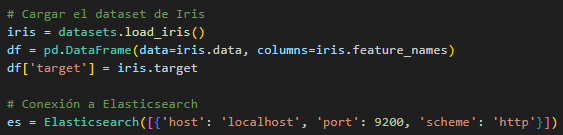
\includegraphics[width=1\linewidth]{img/iris1.png}
    \caption{Parte inicial del primer script de Machine Learning.}
    \label{fig:script11}
\end{figure}

En la segunda parte del primer script se va a definir tanto el nombre del índice que contendrá el \textit{dataset} Iris como el nombre de las propiedas del mismo junto con el tipo que son \ref{fig:script12}, de manera que coincidan con las del \textit{dataset} original para que no haya errores. 

\begin{figure}
    \centering
    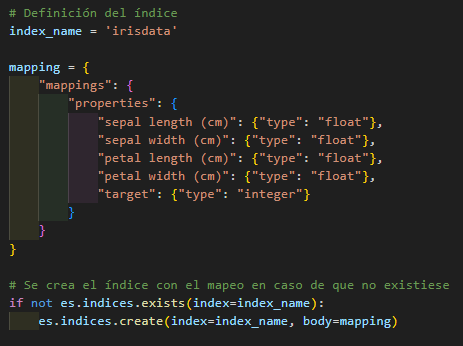
\includegraphics[width=1\linewidth]{img/iris2.png}
    \caption{Segunda parte del primer script de Machine Learning}
    \label{fig:script12}
\end{figure}

Una vez se tiene toda la información del destino de los datos cargada, se procede al envío de los mismos \ref{fig:script13} de manera que se vayan mostrando por pantalla en la terminal a medida que van siendo cargados.

\begin{figure}
    \centering
    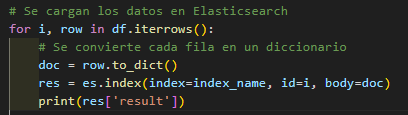
\includegraphics[width=1\linewidth]{img/iris3.png}
    \caption{Parte final del primer script de Machine Learning.}
    \label{fig:script13}
\end{figure}

\paragraph{}
\paragraph{}
\paragraph{}
\paragraph{}


Tras ejecutar este primer script los datos ya están presentes en Elastic, y para fragmentar el trabajo se creó un segundo script en el que se trabajara sobre esos datos cargados. En este segundo script lo primero que se hacer es definir tanto la función \textit{load data from elasticsearch} como \textit{create index} que lo que van a hacer es facilitar la carga de datos del índice que se le indique pasado por valor, y crear nuevos índices con los nombres indicados \ref{fig:script21}. Están son funciones auxiliares en futuros pasos del script.


\begin{figure}
    \centering
    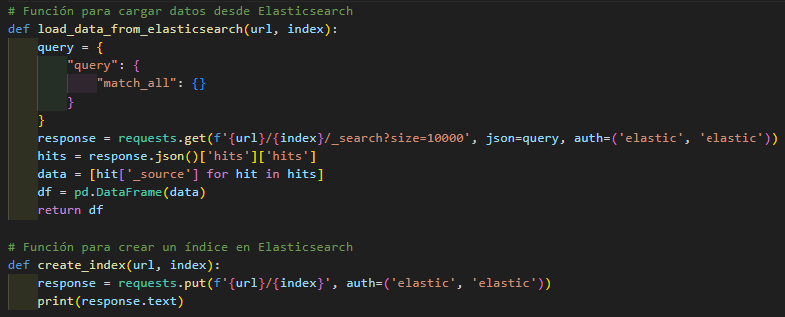
\includegraphics[width=1\linewidth]{img/iris4.png}
    \caption{Definición de funciones auxiliares para el segundo script de Machine Learning.}
    \label{fig:script21}
\end{figure}

En la segunda parte del script se van a seguir realizando operaciones auxiliares para poder operar con los algoritmos. Se establece la URL y el nombre del índice a cargar, que es el mismo en el que se ingestaron los datos de Iris en el script previo, de manera que los datos sean cargados y separados para poder trabajar sobre ellos. También se generan los distintos índices que contendrán los datos obtenidos como resultado de la ejecución de cada algoritmo.

\begin{figure}
    \centering
    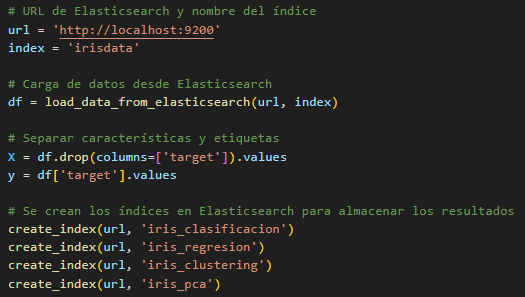
\includegraphics[width=1\linewidth]{img/iris5.png}
    \caption{Definición de operaciones auxiliares y carga de datos para el segundo script de Machine Learning.}
    \label{fig:script22}
\end{figure}

Una vez está toda la información cargada y lista para ser usada, se comienza por el primer algoritmo utilizado, que va a ser uno de clasificación, concretamente \textit{KNN} o K vecinos más cercanos, en el cuál mediante los métodos proporcionados por SKLearn como \textit{train test split}  o \textit{fit}, se creará y entrenará un clasificador en función de los tres vecinos más cercanos \ref{fig:clasificacion1}, obteniendo así una precisión para este clasificador la cuál será exportada a Elastic así como todos los datos que se han procesado en la ejecución del algoritmo, que irán destinados al índice \textit{iris clasificacion} para su posterior uso y exposición en Kibana \ref{fig:clasificacion2}. 

\begin{figure}
    \centering
    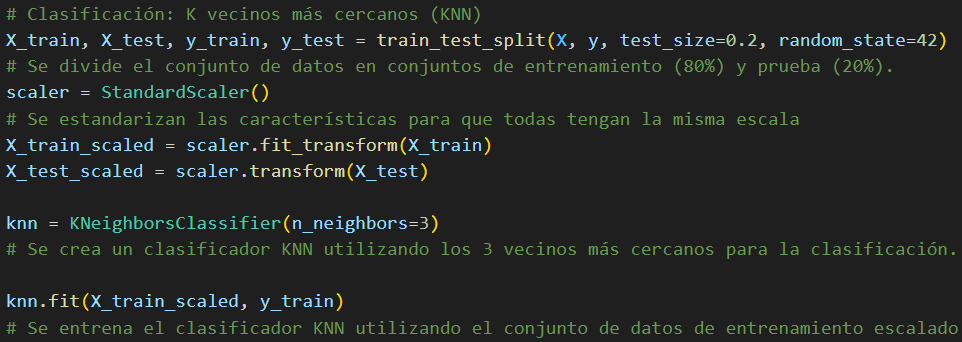
\includegraphics[width=1\linewidth]{img/iris6.png}
    \caption{Generación del clasificador y entrenamiento.}
    \label{fig:clasificacion1}
\end{figure}
\begin{figure}
    \centering
    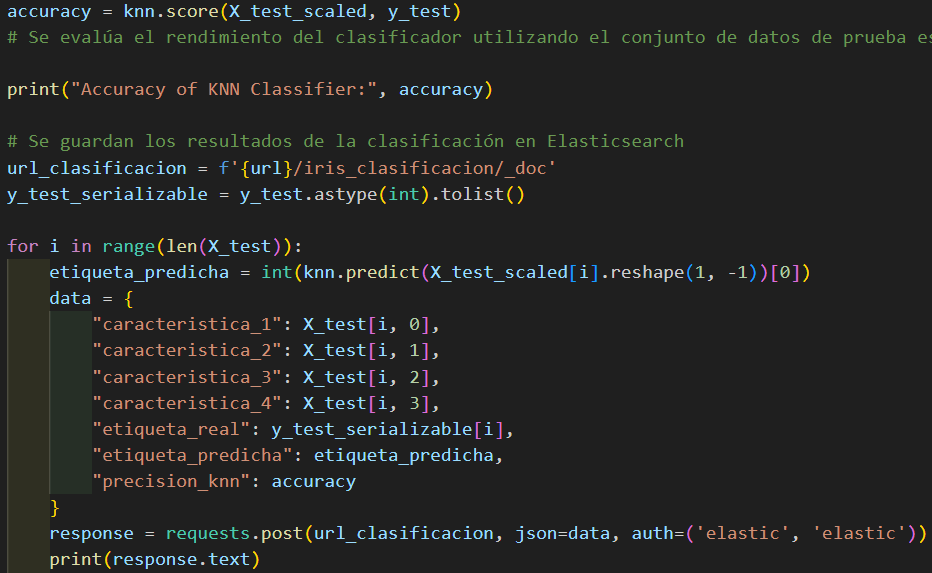
\includegraphics[width=1\linewidth]{img/iris7.png}
    \caption{Cálculo de la precisión del clasificador y envío de datos a Elastic.}
    \label{fig:clasificacion2}
\end{figure}

El siguiente algoritmo al que se le ha dado uso es el de regresión lineal, en el cuál tomando como referencia la tercera característica (longitud del pétalo) para el eje X, y la cuarta característica (anchura del pétalo) para el eje Y, se cree un modelo que sea capaz de predecir un comportamiento típico de los datos. Para ello se le entrena mediante el método \textit{fit} con un conjunto de datos de entrenamiento obtenido de los totales \ref{fig:regresion1}. Posteriormente se evalúa su rendimiento y se manda a Elastic junto con el resto de datos empleados al índice \textit{iris regresion} r\ref{fig:regresion2}.
\begin{figure}
    \centering
    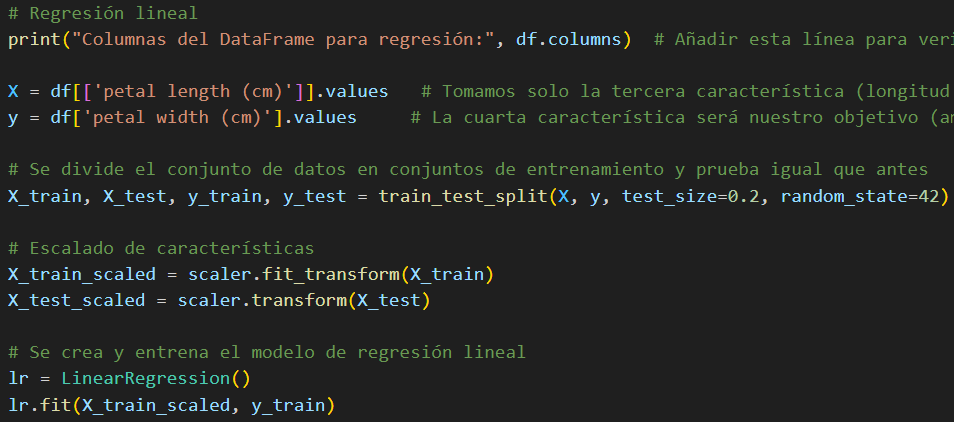
\includegraphics[width=1\linewidth]{img/iris8.png}
    \caption{Generación del modelo de regresión y los conjuntos de entrenamiento.}
    \label{fig:regresion1}
\end{figure}


\begin{figure}
    \centering
    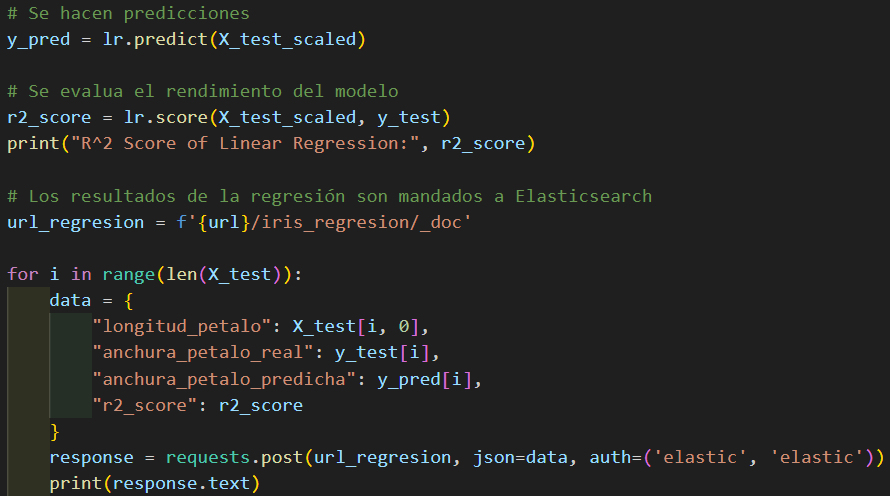
\includegraphics[width=1\linewidth]{img/iris9.png}
    \caption{Cáclulo del rendimiento del modelo y envío de datos a Elastic.}
    \label{fig:regresion2}
\end{figure}


En este tercer algoritmo se va a emplear uno de \textit{clustering}, el \textit{K Means}, en el cuál se van a generar tres clusters de manera que se cree un modelo que devuelva una visualización de los tres en forma de gráfico de dispersión de la longitud y anchura de los sépalos \ref{fig:cluster1}. Una vez se obtiene el gráfico, los datos son mandados a Elastic para poder visualizarlos en un \textit{dashboard}.
\begin{figure}
    \centering
    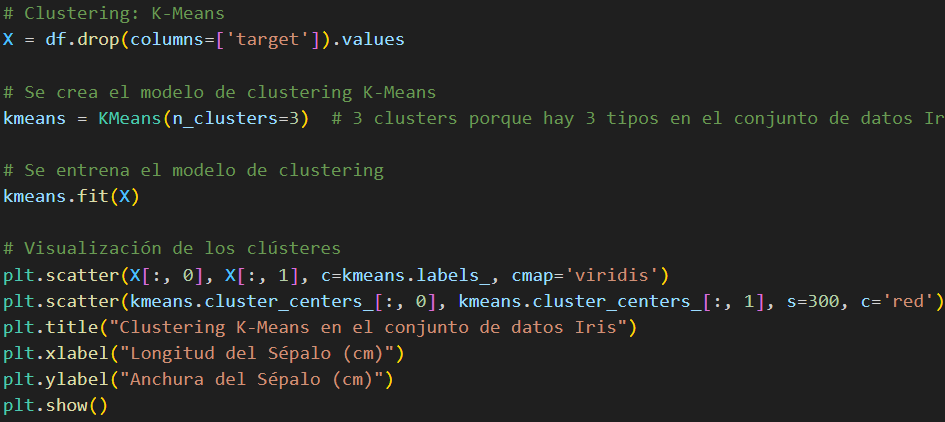
\includegraphics[width=1\linewidth]{img/iris10.png}
    \caption{Estructura del algoritmo \textit{K Means} del segundo script de Machine Learning.}
    \label{fig:cluster1}
\end{figure}

\paragraph{}
\paragraph{}
\paragraph{}

Por último se va a hacer uso de otro algoritmo visual de reducción de dimensionalidad, \textit{PCA}. Al igual que en el anterior, se quiere generar un gráfico bidimensional, por lo que se toman dos componentes equivalentes a los pétalos y sépalos distinguidos por el campo \textit{target} \ref{fig:pca1}. Se entrena el modelo y se genera un gráfico de dispersioón con estos dos componentes el cuál será enviado a Elastic junto con toda la información involucrada. 
\begin{figure}
    \centering
    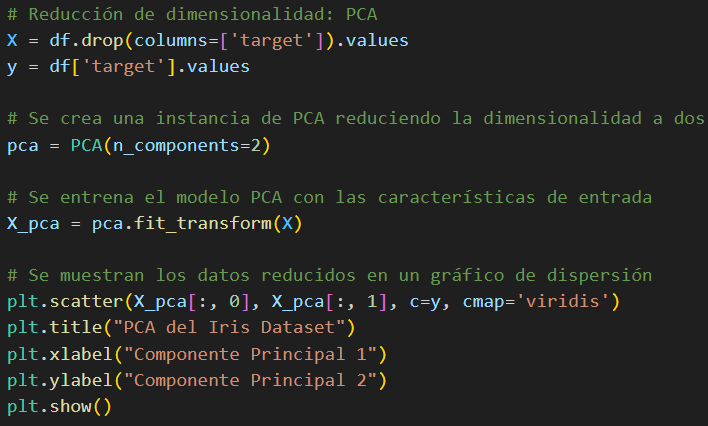
\includegraphics[width=1\linewidth]{img/iris11.png}
    \caption{Estructura del algoritmo de reducción de la dimensionalidad del segundo script de Machine Learning.}
    \label{fig:pca1}
\end{figure}

Tras ejecutar los dos scripts los datos llegarán los diferentes índices que se han ido indicando en ambos. El \textit{dataset} Iris estará almacenado en el índice \textit{irisdata} \ref{fig:index1}, los datos del algoritmo de clasificiación en el índice \textit{iris clasificacion} \ref{fig:index2}, los datos del algoritmo de regresión en el índice \textit{iris regresion} \ref{fig:index3}, los datos del algoritmo de clustering en el índice \textit{iris clustering} \ref{fig:index4},  y por último los datos del algoritmo de reducción de dimensionalidad en el índice \textit{iris pca} \ref{fig:index5}.

\begin{figure}
    \centering
    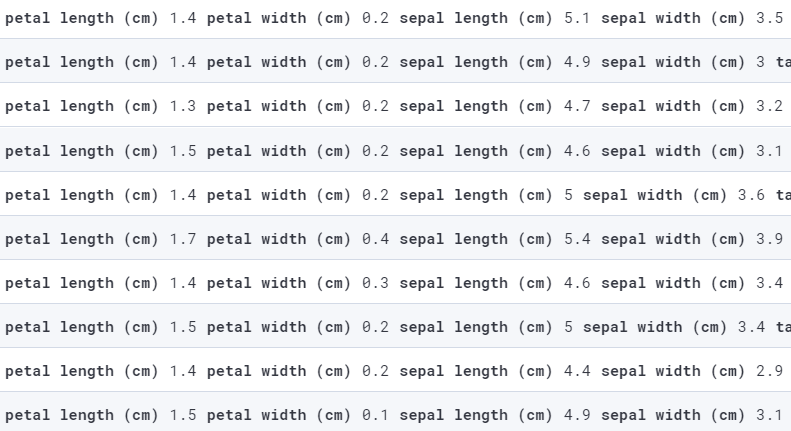
\includegraphics[width=1\linewidth]{img/iris13.png}
    \caption{Índice \textit{irisdata} con información de los datos de Iris.}
    \label{fig:index1}
\end{figure}


\begin{figure}
    \centering
    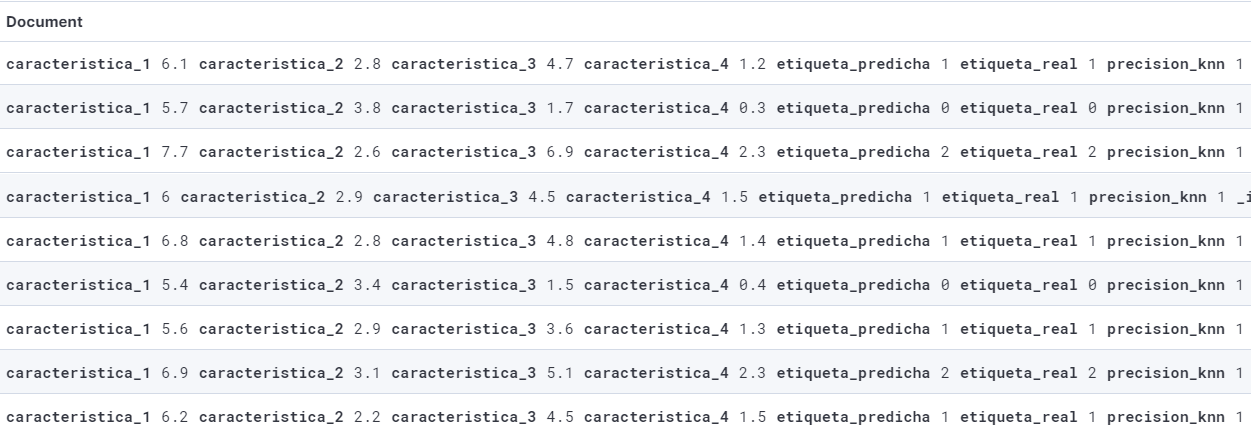
\includegraphics[width=1\linewidth]{img/iris14.png}
    \caption{Índice \textit{iris clasificacion} con información de los datos procesados por el algoritmo de clasificación.}
    \label{fig:index2}
\end{figure}


\begin{figure}
    \centering
    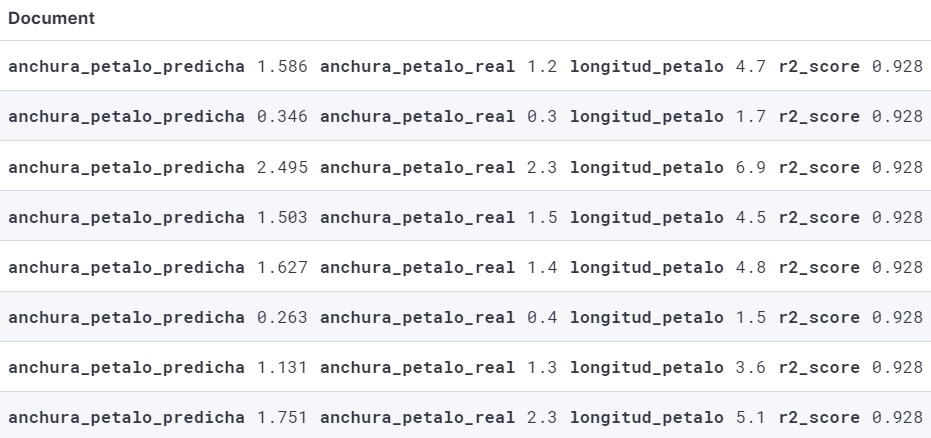
\includegraphics[width=1\linewidth]{img/iris15.png}
    \caption{Índice \textit{iris regresion} con información de los datos procesados por el algoritmo de regresión.}
    \label{fig:index3}
\end{figure}


\begin{figure}
    \centering
    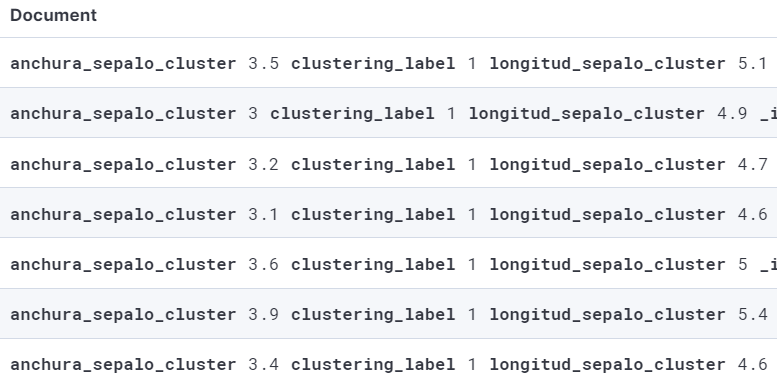
\includegraphics[width=1\linewidth]{img/iris16.png}
    \caption{Índice \textit{iris clustering} con información de los datos procesados por el algoritmo de clustering.}
    \label{fig:index4}
\end{figure}



\begin{figure}
    \centering
    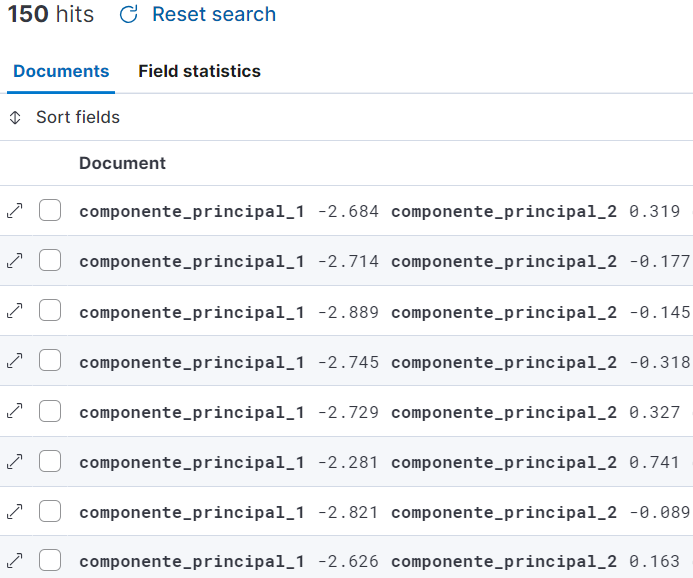
\includegraphics[width=1\linewidth]{img/iris17.png}
    \caption{Índice \textit{iris pca} con información de los datos procesados por el algoritmo de reducción de dimensionalidad.}
    \label{fig:index5}
\end{figure}









